\chapter{\chapternamespectraemission}\label{chap:spectra_emission}

Neste capítulo discutiremos um aspecto interessante observado durante a análise dos espectros das candidatas a UCDs. Durante a inspeção de alguns objetos compactos, identificamos sinais de linhas de emissão nos fotoespectros, especialmente no filtro $J0660$. Esse comportamento pode indicar a presença de H$\alpha$, o que nos levou a investigar mais detalhadamente esses objetos. 

Embora nosso foco principal sejam as galáxias anãs ultracompactas (UCDs), que, por sua natureza, apresentam baixa formação estelar e pouco conteúdo de gás, a detecção de linhas de emissão sugere que esses objetos podem não ser UCDs. Em vez disso, eles podem ser galáxias compactas com formação estelar ativa, possivelmente pertencentes à classe das \ac{BCD}. 

Essa descoberta é relevante, pois amplia nossa compreensão sobre a diversidade de objetos compactos presentes na região estudada. Além disso, a identificação de galáxias compactas com formação estelar ativa pode abrir novas possibilidades para estudos futuros.

Assim, como estava fora do escopo principal do projeto, nesta seção apresentaremos alguns resultados preliminares desses objetos, selecionados para o pedido de tempo de observação descrito na subseção \ref{section:candidatas_emissao}. Os resultados das reduções dos espectros são apresentados na subseção \ref{section:resultado_espectros_emissao}, onde confirmamos a presença de linhas de emissão. Dessa forma, também mostramos um resultado inicial da seleção desses objetos compactos a partir da fotometria do S-PLUS, detalhada na subseção \ref{subsec:candidatas_emissao}. Este processo demonstra a eficácia da metodologia adotada para identificar objetos compactos com características específicas, mesmo que estejam fora do intervalo de redshift esperado para o aglomerado de Fornax.

\section{Seleção da amostra com sinais de linhas de emissão}\label{section:candidatas_emissao}
Nesta seção apresentamos nossa estratégia para identificar objetos compactos com linhas de emissão com a ferramenta Astroinspect \citep{astroinspect}. Podemos fornecer uma tabela de objetos, e ela nos retorna, por exemplo, o \textit{Photo Spec}, isto é, uma imagem do espectro do objeto a partir das medições dos filtros fotométricos do S-PLUS.

Nosso objetivo inicial foi, dentro da amostra de candidatas compactas, encontrar aquelas cujo \textit{Photo Spec} apresentassem um salto nas medições do filtro $J0660$. Esse salto poderia indicar a presença de linhas de emissão de H$\alpha$ (esperadas para esse filtro em repouso), o que seria um indicativo de que, dado o redshift baixo de Fornax, poderíamos estar observando objetos dentro do intervalo de redshifts compatíveis com o aglomerado. Ou seja, se existir algum objeto com emissões em H$\alpha$ em Fornax, é esperado observar um salto no filtro $J0660$.

A partir de uma lista inicial de candidatas, selecionamos visualmente seis objetos promissores que apresentavam sinais de linhas de emissão para fazer um pedido de espectroscopia. Na Figura \ref{candidatas_espectroscopia_2_img}, apresentamos as imagens desses objetos. Na Figura \ref{photo_spec_candidatas}, apresentamos os \textit{Photo Specs} desses objetos, gerados com a ferramenta Astroinspect.


\begin{figure}[!ht]
    \centering
    \captionsetup{justification=centering}
    \begin{subfigure}[b]{0.25\textwidth}
        \includegraphics[width=\textwidth]{proposatal_candidatas_2/Candidate_1.png}
        \caption{Candidate\_1}
    \end{subfigure}
    \begin{subfigure}[b]{0.25\textwidth}
        \includegraphics[width=\textwidth]{proposatal_candidatas_2/Candidate_2.png}
        \caption{Candidate\_2}
    \end{subfigure}
    \begin{subfigure}[b]{0.25\textwidth}
        \includegraphics[width=\textwidth]{proposatal_candidatas_2/Candidate_3.png}
        \caption{Candidate\_3}
    \end{subfigure}
    \begin{subfigure}[b]{0.25\textwidth}
        \includegraphics[width=\textwidth]{proposatal_candidatas_2/Candidate_4.png}
        \caption{Candidate\_4}
    \end{subfigure}
    \begin{subfigure}[b]{0.25\textwidth}
        \includegraphics[width=\textwidth]{proposatal_candidatas_2/Candidate_5.png}
        \caption{Candidate\_5}
    \end{subfigure}
    \begin{subfigure}[b]{0.25\textwidth}
        \includegraphics[width=\textwidth]{proposatal_candidatas_2/Candidate_6.png}
        \caption{Candidate\_6}
    \end{subfigure}
    \caption{Imagens das candidatas a objetos compactos com sinais de linhas de emissão no filtro $J0660$. Imagens obtidas pelo Legacy Survey. Os nomes correspondem ao nome interno usado para o pedido de tempo de observação espectroscópica no Gemini..}
    \label{candidatas_espectroscopia_2_img}
\end{figure}

\begin{figure}[!ht]
    \centering
    \captionsetup{justification=centering}
    \begin{subfigure}[b]{0.3\textwidth}
        \includegraphics[width=\textwidth]{photo_specs/Candidate_1.png}
        \caption{Candidate\_1}
    \end{subfigure}
    \begin{subfigure}[b]{0.3\textwidth}
        \includegraphics[width=\textwidth]{photo_specs/Candidate_2.png}
        \caption{Candidate\_2}
    \end{subfigure}
    \begin{subfigure}[b]{0.3\textwidth}
        \includegraphics[width=\textwidth]{photo_specs/Candidate_3.png}
        \caption{Candidate\_3}
    \end{subfigure}
    \begin{subfigure}[b]{0.3\textwidth}
        \includegraphics[width=\textwidth]{photo_specs/Candidate_4.png}
        \caption{Candidate\_4}
    \end{subfigure}
    \begin{subfigure}[b]{0.3\textwidth}
        \includegraphics[width=\textwidth]{photo_specs/Candidate_5.png}
        \caption{Candidate\_5}
    \end{subfigure}
    \begin{subfigure}[b]{0.3\textwidth}
        \includegraphics[width=\textwidth]{photo_specs/Candidate_6.png}
        \caption{Candidate\_6}
    \end{subfigure}
    \caption{Imagens dos \textit{Photo Spec}, criadas pela Ferramenta Astroinspect \cite{astroinspect}, das candidatas a objetos compactos com sinais de linhas de emissão no filtro $J0660$. Os nomes correspondem ao nome interno usado para o pedido de tempo de observação espectroscópica no Gemini.}
    \label{photo_spec_candidatas}
\end{figure}

Observamos na Figura \ref{photo_spec_candidatas} que os objetos apresentam sinais de linhas de emissão no filtro $J0660$, conforme comentado. Dessa forma, esses objetos foram selecionados para a observação espectroscópica no Gemini Sul.


\section{Observações com o Gemini Sul}\label{section:observacoes_gemini_sul_2}
Para as observações, utilizamos o espectrômetro GMOS no telescópio Gemini Sul. O pedido de tempo foi feito para observarmos 6 objetos, e as observações foram realizadas em 2024.

Para a observação espectroscópica foi utilizado o espectrógrafo GMOS-S montado no telescópio Gemini South, operando em modo Longslit. As principais configurações aplicadas às observações são resumidas abaixo:

\begin{itemize}
    \item \textbf{Modo de Observação}: Fenda longa (\textit{long-slit}).
    \item \textbf{Grating}: B600-G5323, com comprimento de onda central em 3 posições: $\lambda_c = 515 \, \text{nm}$, $\lambda_c = 550 \, \text{nm}$ e $\lambda_c = 585 \, \text{nm}$.
    \item \textbf{Largura da Fenda}: 1".
    \item \textbf{Resolução Espectral}: $R \sim 570$, considerando a largura da fenda escolhida.
    \item \textbf{Intervalo Espectral}: 4000\,\text{Å} a 7000\,\text{Å}.
    \item \textbf{Condições de Observação}: IQ=85\%, CC=70\%, WV=ANY, SB=80\%.
    \item \textbf{Razão Sinal-Ruído (S/N) Desejada}: Mínimo de 3 no espectro combinado no contínuo, suficiente para detectar o declive do contínuo azul e as principais linhas de absorção.
    \item \textbf{Número de Exposições}: Em cada comprimento de onda central, 1 exposição de 600 segundos cada, totalizando 3 exposições por objeto.
\end{itemize}

O processo de redução dos dados espectroscópicos foi realizado seguindo as mesmas etapas descritas no apêndice \ref{sec:reducao}.

\section{Resultados}\label{section:resultado_espectros_emissao}

Tivemos seis candidatas observadas neste projeto. Os espectros desses objetos, depois de limparmos os artefatos, são apresentados na Figura \ref{espectros_candidatas_2}.

\begin{figure}[!ht]
    \centering
    \captionsetup{justification=centering}
    \begin{subfigure}[b]{0.45\textwidth}
        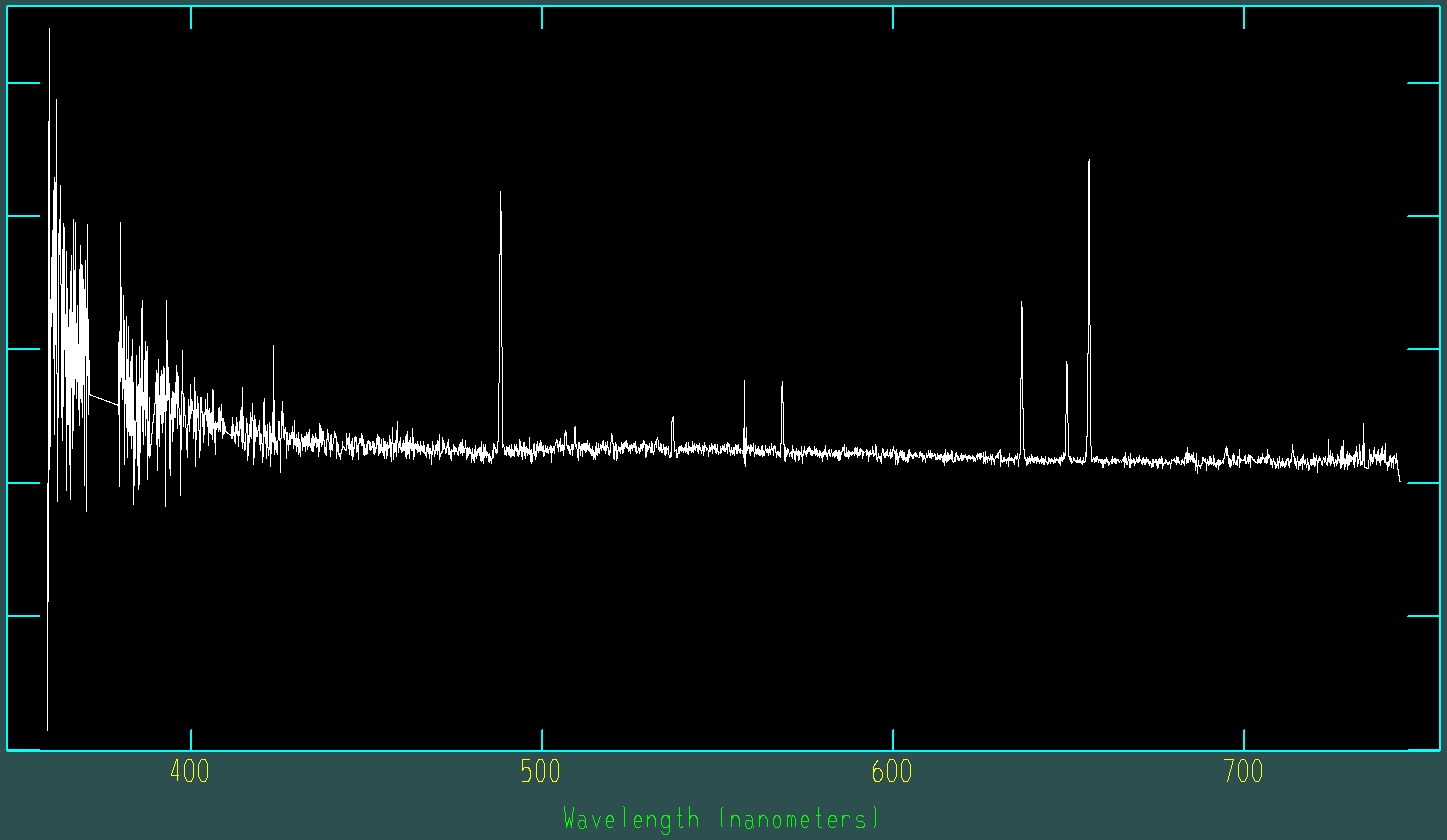
\includegraphics[width=\textwidth]{espectros/Candidate1.png}
        \caption{Candidate1}
    \end{subfigure}
    \begin{subfigure}[b]{0.45\textwidth}
        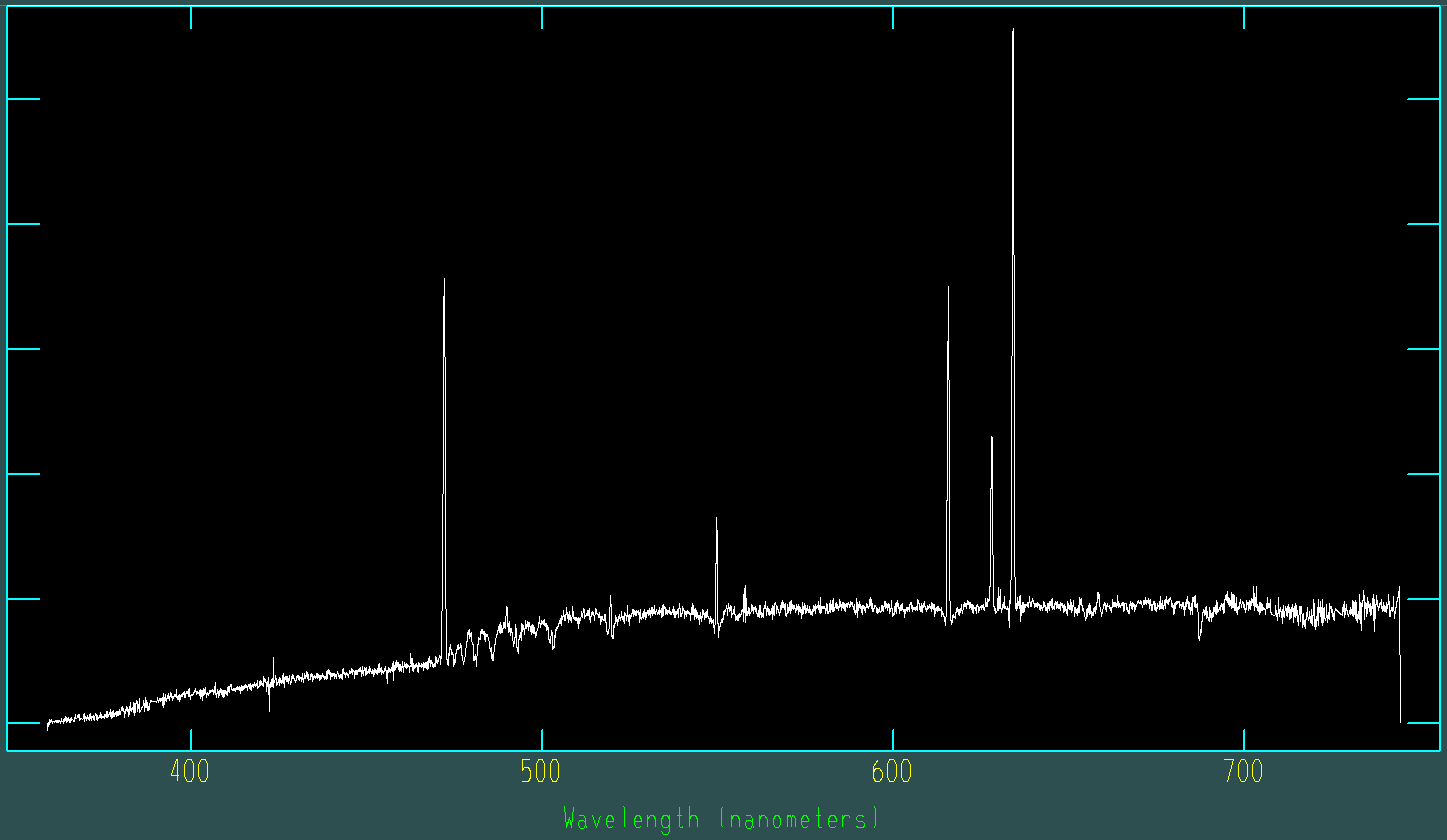
\includegraphics[width=\textwidth]{espectros/Candidate2.png}
        \caption{Candidate2}
    \end{subfigure}
    \begin{subfigure}[b]{0.45\textwidth}
        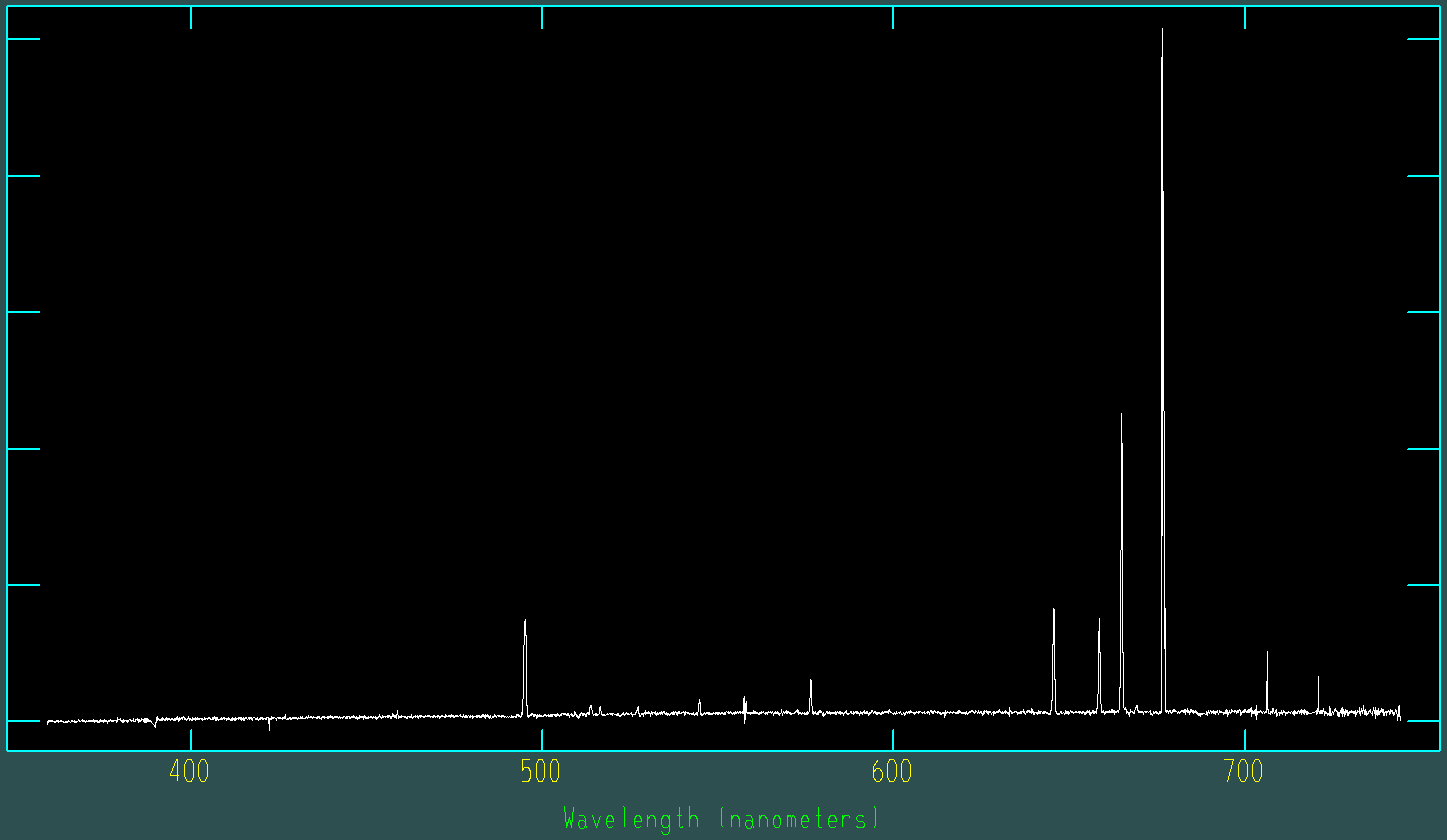
\includegraphics[width=\textwidth]{espectros/Candidate3.png}
        \caption{Candidate3}
    \end{subfigure}
    \begin{subfigure}[b]{0.45\textwidth}
        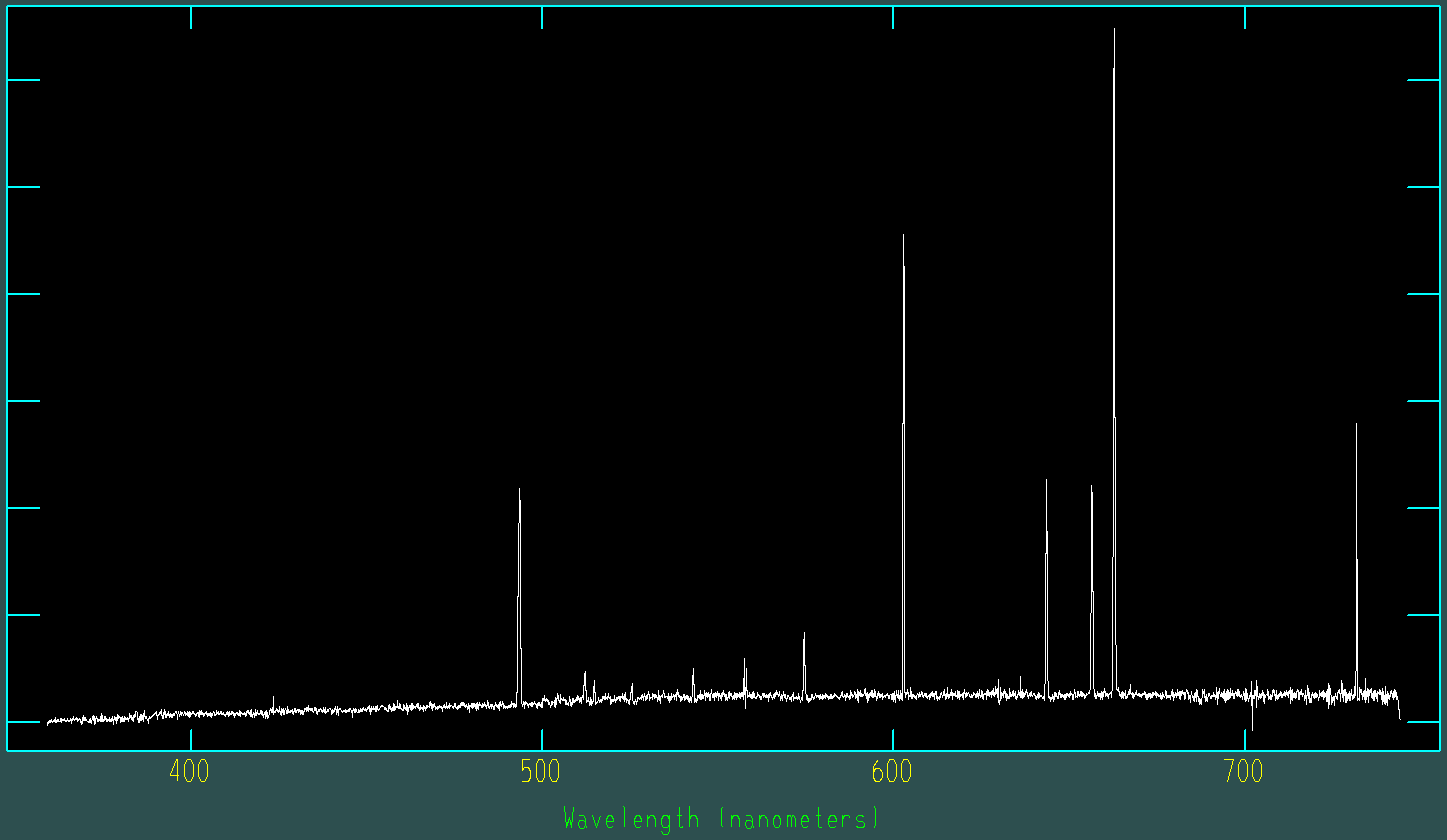
\includegraphics[width=\textwidth]{espectros/Candidate4.png}
        \caption{Candidate4}
    \end{subfigure}
    \begin{subfigure}[b]{0.45\textwidth}
        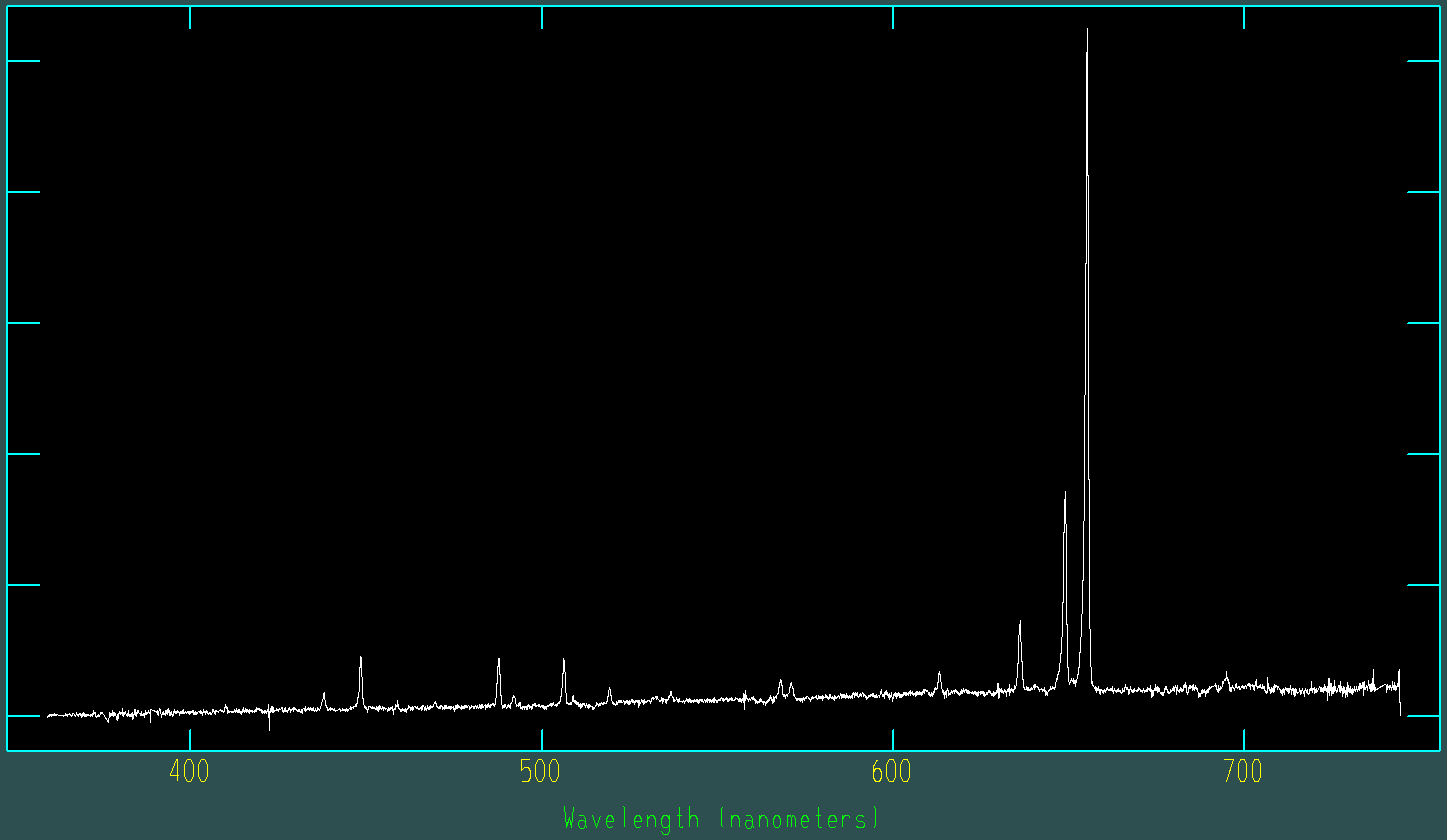
\includegraphics[width=\textwidth]{espectros/Candidate5.png}
        \caption{Candidate5}
    \end{subfigure}
    \begin{subfigure}[b]{0.45\textwidth}
        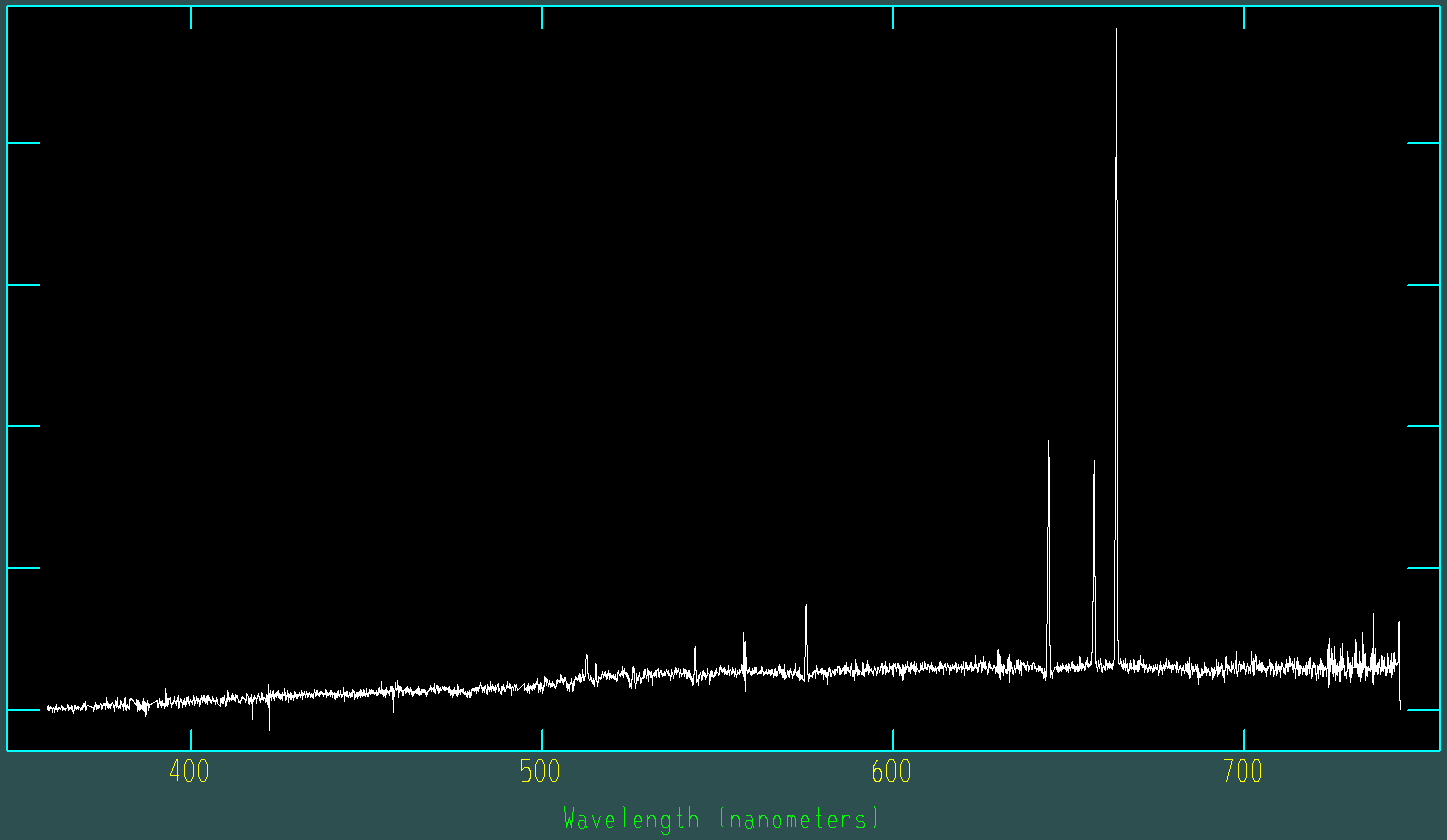
\includegraphics[width=\textwidth]{espectros/Candidate6.png}
        \caption{Candidate6}
    \end{subfigure}
    \caption{Espectros das candidatas com sinais de linhas de emissão no filtro $J0660$ observadas no Gemini Sul. Os nomes correspondem ao nome interno usado para o pedido de tempo de observação.}
    \label{espectros_candidatas_2}
\end{figure}

Analisando cada espectro e as linhas de emissão presentes, mostramos na Tabela \ref{redshift_candidatas_2} os redshifts obtidos para cada objeto, após a identificação de pelo menos duas linhas e o deslocamento em relação ao repouso.

\begin{table}[!ht]
    \centering
    \caption{Redshifts (\textit{z}) obtidos a partir dos espectros do conjunto de candidatas com sinais de linhas de emissão no filtro $J0660$ observadas com o GMOS no telescópio Gemini Sul. A coluna $OBJ_{name}$ é o nome interno da candidata utilizado no pedido de tempo do Gemini.} 
    \begin{tabular}{lcc}
        \toprule
        $OBJ_{name}$ & z   \\
        \midrule
        Candidate\_1     & 0.309 \\
        Candidate\_2     & 0.265 \\
        Candidate\_3     & 0.327 \\
        Candidate\_4     & 0.323 \\
        Candidate\_5     & 0.308 \\
        Candidate\_6     & 0.325 \\
        \bottomrule
    \end{tabular}
    \label{redshift_candidatas_2}
\end{table}

Todos os objetos mostram sinais de emissão bem definidos, especialmente onde estávamos esperando, no filtro $J0660$. Os redshifts obtidos para esses objetos estão entre 0.265 e 0.327, o que indica que esses objetos estão a uma distância considerável do aglomerado de Fornax.

Nossa ideia inicial era encontrar linhas de emissão, especificamente o $H\alpha$, que indicassem a presença de objetos compactos em Fornax, a partir apenas de uma seleção do nosso modelo com as predições. Porém, os redshifts obtidos para esses objetos indicam que eles estavam no intervalo necessário para observarmos as linhas do dubleto de $[OIII]4959,5007$ no filtro $J0660$. É interessante ressaltar que, mesmo sendo objetos de fundo, eles ainda são consideravelmente compactos, e as fortes presenças de linhas de emissão indicam que podem ser galáxias com formação estelar recente, um tópico interessante que será explorado no doutorado.

Todos os objetos foram caracterizados como galáxias compactas, mostrando assim a eficiência do método de seleção de objetos compactos a partir do modelo treinado. Para a seleção desses objetos, não passamos pelos critérios com cortes nos redshifts fotométricos. Assim, mesmo não selecionando objetos em Fornax, o método de seleção foi eficiente para encontrar objetos compactos com emissão em $z\sim 0.3$, e que a inclusão de critérios de redshifts fotométricos permite refinar ainda mais a busca.

% Os resultados dos espectros desses objetos, por si só, são interessantes, visto que são objetos compactos, bem azuis, com formação estelar recente e presença de fortes linhas de emissão. Vemos na Figura \ref{redshift_candidatas_2}, para todos os objetos, a presença de diversas linhas de emissão. Na \textit{Candidate5}, por exemplo, encontramos sinais das linhas de emissão de Ne \textsc{v}, Ne \textsc{vi}, [O \textsc{ii}], He \textsc{i}, [S \textsc{ii}], H$\delta$, H$\gamma$, [O \textsc{iii}], H$\beta$, [O \textsc{iii}].

Os resultados dos espectros desses objetos, por si só, são interessantes, visto que são objetos compactos, bem azuis, com formação estelar recente e presença de fortes linhas de emissão. Vemos na Figura \ref{redshift_candidatas_2}, para todos os objetos, a presença de diversas linhas de emissão. Na \textit{Candidate5}, por exemplo, encontramos sinais das linhas de emissão de Ne \textsc{v} $\lambda3426$, Ne \textsc{vi} $\lambda3346$, [O \textsc{ii}] $\lambda3727$, He \textsc{i} $\lambda5876$, [S \textsc{ii}] $\lambda6717$, H$\delta$, H$\gamma$, [O \textsc{iii}] $\lambda4959$, H$\beta$, [O \textsc{iii}] $\lambda5007$.

Nosso método foi capaz de recuperar galáxias compactas. Mesmo com essa pré-seleção de objetos que não estavam no aglomerado de Fornax, encontramos uma maneira de mapear e identificar objetos interessantes para estudos futuros. Em especial, concluímos que podemos encontrar objetos em redshifts por volta de 0,3, onde galáxias com fortes linhas de emissão serão evidenciadas pelo filtro estreito $J0660$.

\section{Seleção de novas candidatas com sinais de emissão} \label{subsec:candidatas_emissao}
Os resultados do pedido de observação dessas seis candidatas confirmou que essa estratégia foi eficaz para identificar objetos com sinais de emissão. No entanto, nenhum dos seis objetos observados foi encontrado no redshift do aglomerado de Fornax.

Considerando que a subseleção de objetos compactos com características que evidenciam linhas de emissão sensíveis ao filtro $J0660$ se mostrou eficaz, criamos um critério adicional que destaque esses objetos. Na Figura \ref{ex_photospec_f600}, mostramos o fotoespectro de um dos exemplos das 6 candidatas que foram observadas com sinais de emissão. Notamos como o pico no filtro $J0660$ é evidente quando o comparamos com os dois filtros adjacentes, $r$ e $i$.

\begin{figure}[!ht]
    \begin{center}
    \includegraphics[width=0.85\columnwidth,angle=0]{photo_specs/Candidate_2.png}
    \caption[]{Imagem do \textit{Photo Spec}, criada pela Ferramenta Astroinspect \cite{astroinspect}, da \textit{Candidate\_2} da lista de candidatas da subseção \ref{section:candidatas_emissao} de objetos compactos com sinais de linhas de emissão no filtro $J0660$.}
    \label{ex_photospec_f600}
    \end{center}
\end{figure}

Testamos criar uma seleção em cores com esses 3 filtros que destacassem esses objetos. A cor que iremos adotar é a diferença do filtro central, $J0660$, com a média dos filtros adjacentes, $r$ e $i$. Assim, esperamos que objetos com maiores picos tenham essa cor mais destoante. A cor adotada é a seguinte:

\begin{equation}
    \text{Color\_HAlpha} = J0660 - \frac{r + i}{2}
    \label{equantion_halpha_color}
\end{equation}

% Demonstrando como essa cor utilizada pode destacar essa característica, criamos um gráfico contendo parte dos objetos da nossa amostra classificados como estrela ou galáxia, comparados com os 6 objetos com sinais de emissão que encontramos anteriormente. Na Figura \ref{color_halpha}, mostramos a distribuição dessa cor para esses objetos.

% \begin{figure}[!ht]
%     \begin{center}
%     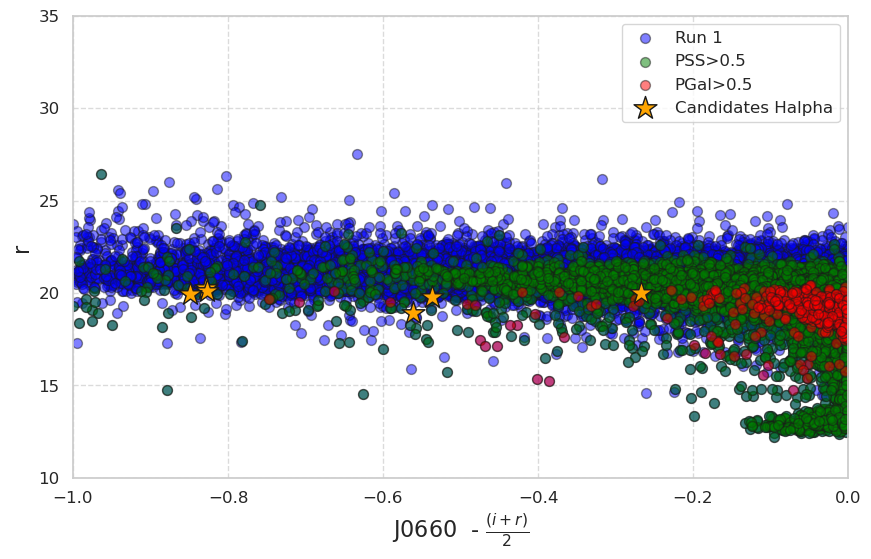
\includegraphics[width=1.\columnwidth,angle=0]{color_halpha.png}
%     \caption[]{Gráfico da cor \text{Color\_HAlpha} em função da magnitude \textit{r\_APER\_6}. Pontos em azul são todos os dados da amostra de Fornax. Pontos em verde e vermelho são os objetos classificados como galáxias ou estrelas pelo GAIA DR3, respectivamente. Estrelas em amarelo são os 6 objetos com sinais de emissão que foram observados.}
%     \label{color_halpha}
%     \end{center}
% \end{figure}

Os 6 objetos com sinais de emissão se destacam a partir de um corte em \text{Color\_HAlpha}$\leq$-0.2. Vale ressaltar que, devido aos erros nos filtros e às diferenças entre as bandas $r$, $i$ e $J0660$, não necessariamente objetos com essa cor abaixo desse valor são representativos de terem um pico em $J0660$. Existem casos onde essa cor pode ser intensa devido a uma diferença brusca, de uma grande subida ou descida entre o filtro $i$ e $J0660$ ou $r$ e $J0660$, e não um pico propriamente dito. Então, mesmo sendo capaz de filtrar esses objetos, ainda precisamos avaliar visualmente os fotoespectros.

Da amostra teste para candidatas com alta probabilidade de serem objetos extensos, selecionadas durante as análises apresentadas na seção \ref{sec:selecao_candidatas}, aplicamos um corte de \text{Color\_HAlpha}$\leq$-0.3, para identificar objetos com sinais de emissão. Mostramos na Figura \ref{halpha_candidatas_final} o fotoespectro de 4 exemplo de objetos que foram selecionados com essa cor.

\begin{figure}[!ht]
    \centering
    \captionsetup{justification=centering}
    \begin{subfigure}[b]{0.45\textwidth}
        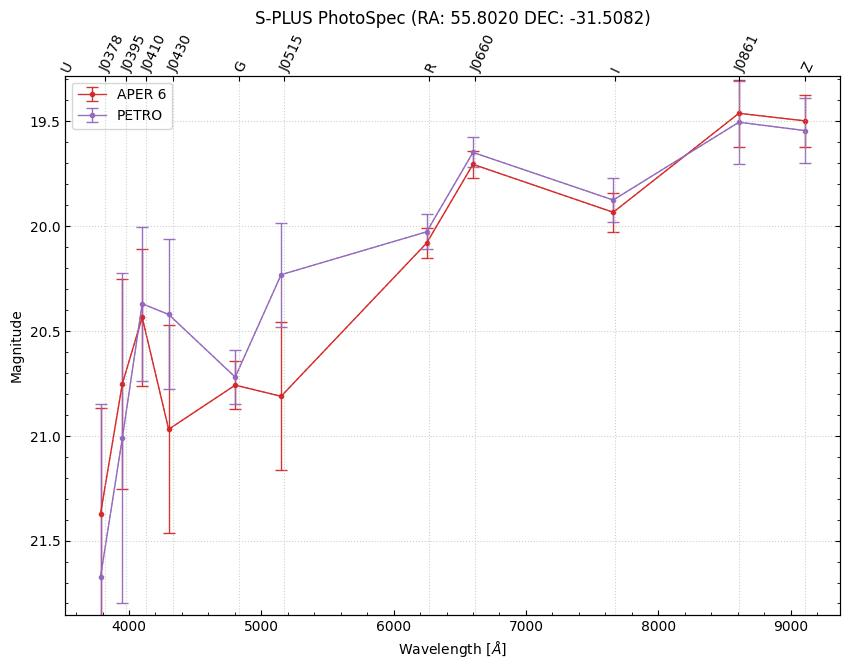
\includegraphics[width=\textwidth]{photo_specs/candidate_final/candidate_final_1.png}
        \caption{a)}
    \end{subfigure}
    \begin{subfigure}[b]{0.45\textwidth}
        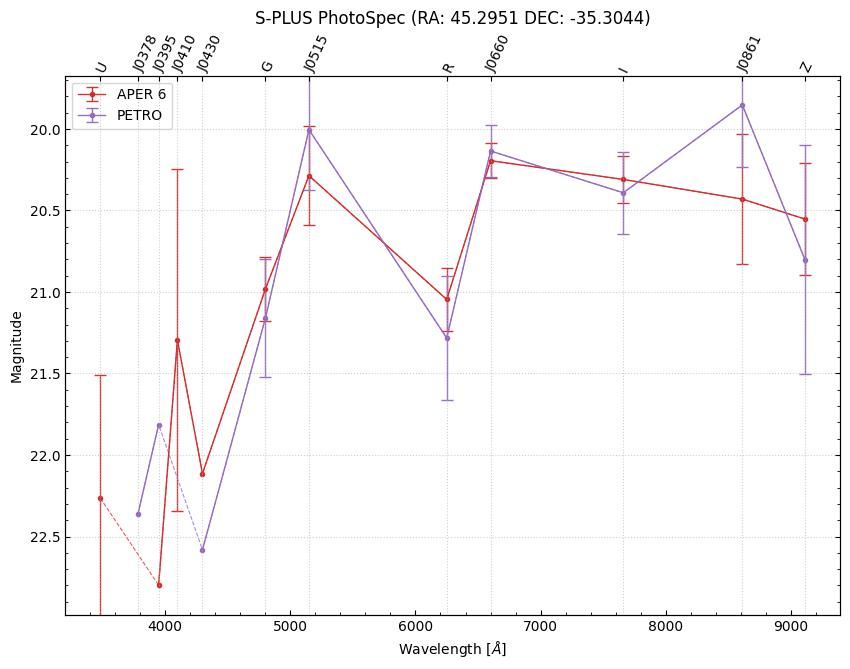
\includegraphics[width=\textwidth]{photo_specs/candidate_final/candidate_final_2.png}
        \caption{b)}
    \end{subfigure}
    \begin{subfigure}[b]{0.45\textwidth}
        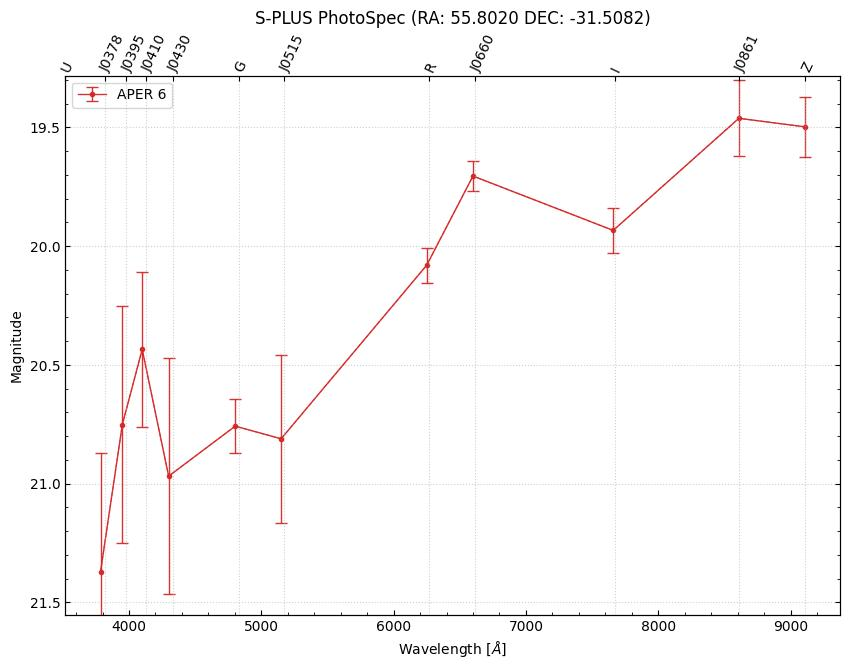
\includegraphics[width=\textwidth]{photo_specs/candidate_final/candidate_final_3.png}
        \caption{c)}
    \end{subfigure}
    \begin{subfigure}[b]{0.45\textwidth}
        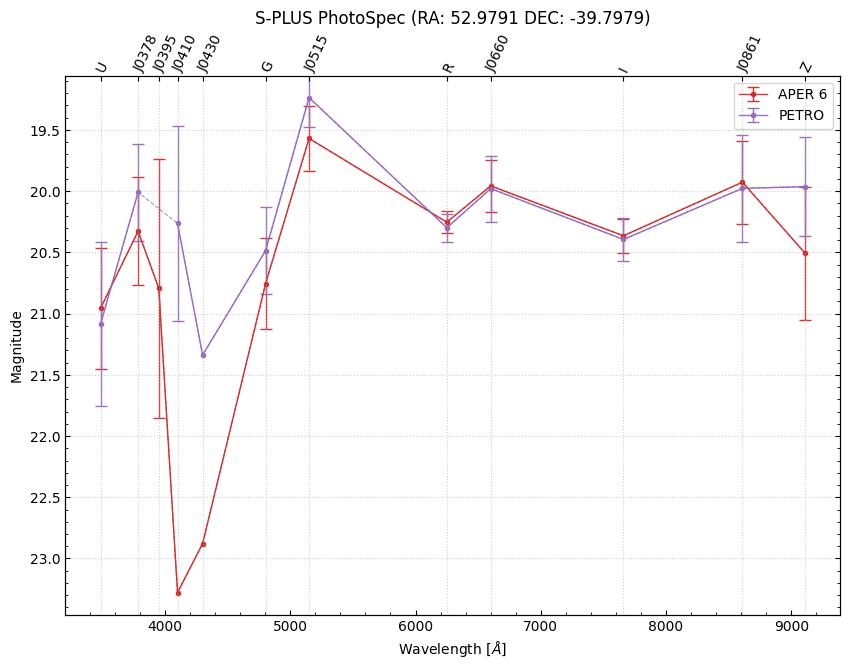
\includegraphics[width=\textwidth]{photo_specs/candidate_final/candidate_final_4.png}
        \caption{d)}
    \end{subfigure}
    \caption{Imagens dos \textit{Photo Spec}, criadas pela Ferramenta Astroinspect \cite{astroinspect}, com corte na cor criada pela equação \ref{equantion_halpha_color}, aplicando um corte abaixo de -0.3 na lista de candidatas finais a objetos compactos de Fornax da seção \ref{sec:selecao_candidatas}.}
    \label{halpha_candidatas_final}
\end{figure}

Concluímos que a metodologia de seleção de objetos compactos foi eficaz em identificar objetos com características interessantes, mesmo em intervalos de redshift em torno de 0.3. Esses objetos podem ser explorados em projetos futuros, especialmente devido à presença de fortes linhas de emissão, que indicam formação estelar ativa.

Além disso, ao final do processo, identificamos uma lista de quatro objetos que podem ser relevantes para estudos futuros de galáxias compactas com linhas de emissão, selecionados com base em cortes de redshift fotométrico para o aglomerado de Fornax. Embora esses objetos não sejam UCDs, sua natureza compacta e os sinais de emissão observados os tornam candidatos promissores para investigações adicionais, ampliando o escopo de estudos sobre a diversidade de objetos compactos no universo.

